\documentclass[russian,11pt]{article}
\usepackage{cmap}
\usepackage{mathtext}
\usepackage[russian]{babel}
\usepackage[a4paper, left=2.00cm, right=2.00cm, top=2.00cm, bottom=2.00cm, marginparwidth=1.75cm]{geometry}
\usepackage{amsmath}
\usepackage{amssymb}
\usepackage{multirow}
\usepackage{fancyhdr}
\usepackage{graphicx}
\usepackage{wrapfig}
\usepackage{array}
\usepackage[sorting=none]{biblatex}
\addbibresource{references.bib}

\providecommand{\keywords}[1]{
\begin{flushright}
\small	
\textbf{Ключевые слова:} #1
\end{flushright}
}
\providecommand{\header}[1]{
\,
\begin{center}
{\Large \textbf{#1}}
\end{center}
}

\title{\textbf{Навигация и управление в робототехнических системах}}
\author{Студенты 1-го курса бакалавриата КТиУ, СУиР \and Овчинников Н.М., Овчинников П.А., Румянцев А.А., Чебаненко Д.А. \and bsbbbrbc@gmail.com, opavel@internet.ru, myspecialuseracc@gmail.com, dchebanenko@gmail.com \and Университет ИТМО, Россия, Санкт-Петербург}
\date{30 мая 2023 г.}
\pagestyle{fancy}
\fancyhf{}
\fancyhead[L]{Навигация и управление в робототехнических системах}
\fancyfoot[C]{\thepage}
\begin{document}
\maketitle
\begin{abstract}
\begin{center}
Научная работа посвящена изучению и анализу различных аспектов навигации и управления в робототехнических системах. Работа включает в себя исследование нейронных сетей для обнаружения объектов в задаче управления автономным транспортным средством, анализ алгоритмов траекторного управления роботом манипулятором, разработку методики планирования траектории движения группы мобильных роботов в неизвестной замкнутой среде с препятствиями, исследование навигации мобильного робота на основе методов лазерной дальномерии, изучение силомоментного ощущения электромеханического манипулятора и анализ траекторного управления мобильным роботом в условиях неопределенности.
\end{center}
\end{abstract}
\keywords{навигация, управление, нейронные сети, \\ робототехника, алгоритмы, траектория движения}
\header{Введение}

В современном мире робототехнические системы играют всё более важную роль в различных сферах жизни, от промышленности до медицины и транспорта. Одними из ключевых аспектов, которые обеспечивают эффективное функционирование роботов, являются навигация и управление. Исследование и разработка методов, алгоритмов и технологий в этой области позволяет создавать более умные, автономные и надежные робототехнические системы.

Целью этой научной работы является изучение и анализ различных областей навигации и управления в робототехнических системах. Мы рассмотрим следующие темы:
\begin{enumerate}
\item \textbf{Исследование алгоритмов траекторного управления роботом-манипулятором.} \\Изучим различные методы и подходы к планированию и управлению траекториями движения манипуляторов, что улучшит точность и эффективность выполнения задач.
\item \textbf{Методика планирования траектории движения группы мобильных роботов в неизвестной замкнутой среде с препятствиями.} Исследуем проблему планирования оптимальных траекторий для группы роботов в условиях ограниченного пространства и наличия препятствий, что крайне важно для координации и сотрудничества роботов в различных задачах.
\item \textbf{Траекторное управление мобильным роботом в условиях неопределенности.} Рассмотрим методы и алгоритмы для планирования и управления траекторией движения мобильного робота в условиях, когда информация о среде ограничена или не определена.
\item \textbf{Навигация мобильного робота на основе методов лазерной дальномерии.} Будет исследовано использование лазерных дальномеров для определения окружающей среды и навигации мобильных роботов, что является одним из ключевых аспектов автономности и безопасности робототехнических систем.
\item \textbf{Силомоментное ощущение электромеханического манипулятора.} Исследуем применение силомоментного ощущения для контроля и управления движениями электромеханического манипулятора, что повысит его гибкость и точность выполнения задач.
\item \textbf{Исследование нейронных сетей для обнаружения объектов в задаче управления автономным транспортным средством.} Исследуем применение нейронных сетей в обнаружении и распознавании объектов на дороге, что является важным шагом в разработке автономных транспортных средств.
\end{enumerate}
\header{Исследование алгоритмов траекторного управления
роботом-манипулятором \cite{1}}

В статье рассматривается задача траекторного управления трехзвенным роботом-манипуля-тором. Авторы исследуют четыре различные схемы управления и сравнивают их работу при наличии различных видов помех. Они пришли к выводу, что первая и четвертая схемы управления являются наиболее эффективными и что наилучший выбор схемы управления зависит от типа присутствующих помех.

Вот краткое изложение четырех схем управления, рассмотренных в статье:
\begin{itemize}
\item \textbf{Пропорционально-дифференциальное (PD) управление} --- 
это простая и часто используемая схема управления, которая эффективна при отсутствии помех. Однако он может быть неустойчивым при наличии шума или параметрической неопределенности.
\item \textbf{Управление в скользящем режиме} --- это более сложная схема управления, более устойчивая к шуму и параметрической неопределенности. Однако она может быть менее плавной, чем управление PD.
\item \textbf{Управление PD с фильтрацией нижних частот} --- это вариант управления PD, в котором для сглаживания управляющего сигнала используется фильтр нижних частот. Это может улучшить динамическую производительность системы, но также может снизить ее быстродействие.
\item \textbf{Адаптивное управление} --- это схема управления, которая автоматически регулирует свои параметры, чтобы компенсировать изменения в системе. Это может сделать систему более устойчивой к шуму и параметрической неопределенности. Однако адаптивное управление может быть более сложным и дорогостоящим в вычислительном отношении, чем другие схемы управления.
\end{itemize}

Авторы статьи провели имитационное исследование для сравнения производительности четырех схем управления в различных условиях. Они обнаружили, что схема управления PD хорошо работала в отсутствие помех, но была нестабильной в присутствии шума или параметрической неопределенности. Схема управления скользящим режимом была более устойчивой к шуму и параметрической неопределенности, но менее плавной, чем управление PD. Схема управления частичным разрядом с фильтром нижних частот улучшила динамические характеристики управления частичным разрядом, но снизила чувствительность системы. Схема адаптивного управления была наиболее устойчивой к шуму и параметрической неопределенности, но она также была самой сложной и дорогостоящей в вычислительном отношении.
\pagebreak

\begin{figure}[!h]
\centering
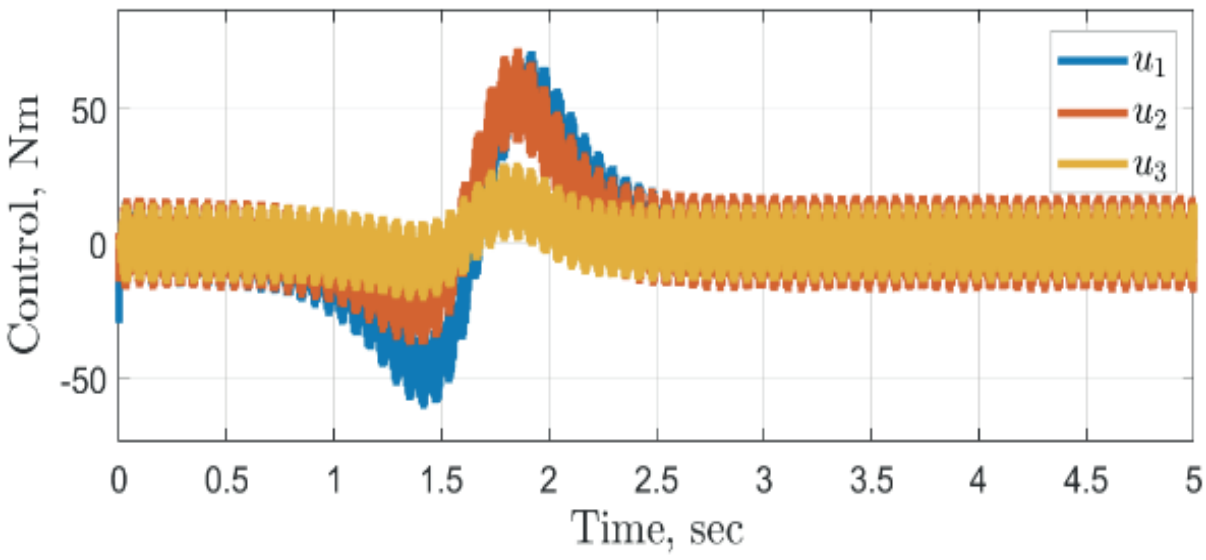
\includegraphics[width=0.4\textwidth]{1_scheme1_harmonic}
\begin{center}{\footnotesize Рис. 1: График управляющего сигнала схемы 1 при помехах \\в виде высокочастотного гармонического сигнала}\end{center}
\end{figure}

\begin{figure}[!h]
\centering
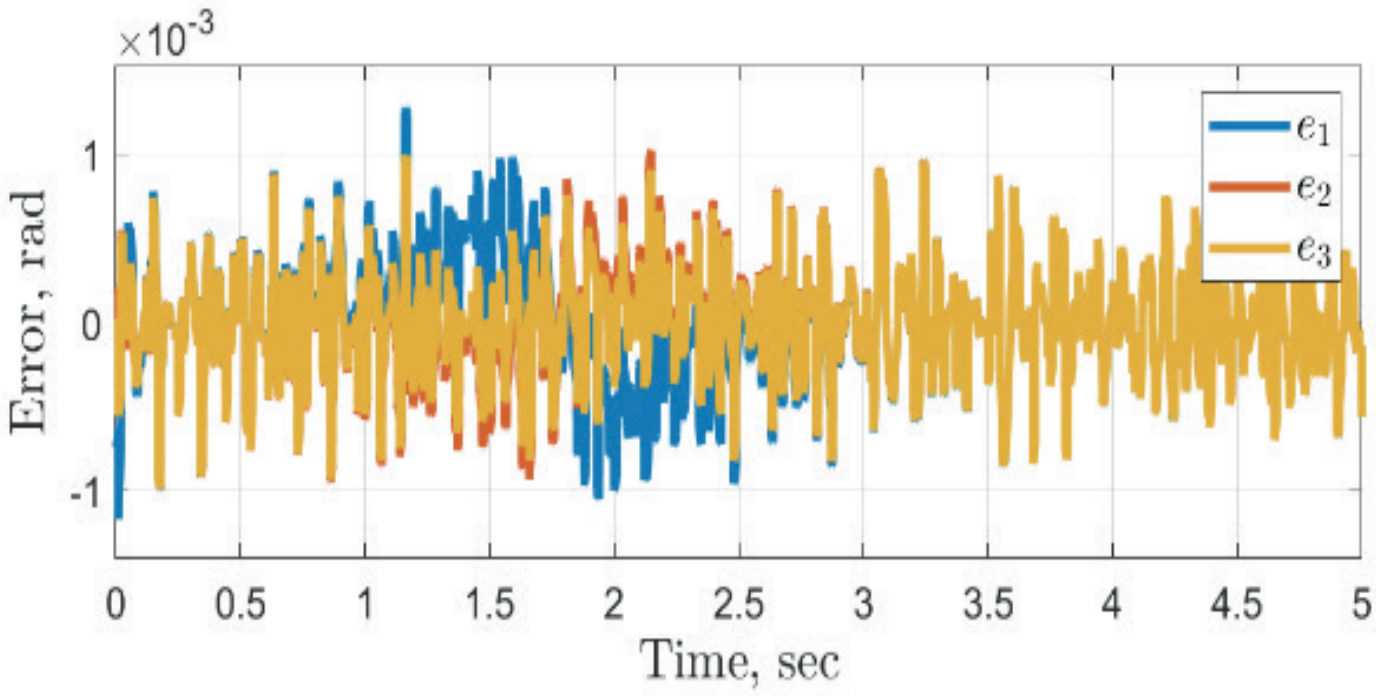
\includegraphics[width=0.4\textwidth]{1_scheme4_noise}
\begin{center}{\footnotesize Рис. 2: График ошибки схемы 4 при помехах в виде белого шума}\end{center}
\end{figure}

По результатам имитационного исследования авторы статьи рекомендуют использовать схему управления PD при отсутствии помех, схему управления скользящим режимом при наличии шума или параметрической неопределенности и схему адаптивного управления в приложениях, где требуется высокая робастность.

Вот еще аргументы в пользу ценности этой статьи:
\begin{itemize}
\item Исследование моделирования авторов дает ценную информацию о производительности четырех схем управления в различных условиях.
\item Рекомендации авторов по выбору схемы управления основаны на надежных теоретических и экспериментальных данных.
\end{itemize}

В целом, статья представляет собой хорошо написанный и информативный вклад в области управления роботами.

\header{Методика планирования траектории движения
группы \\мобильных роботов в неизвестной замкнутой среде \\с препятствиями \cite{2}}

В статье рассматривается метод планирования траектории движения группы мобильных роботов в неизвестной замкнутой среде с препятствиями. Метод основан на децентрализованном подходе, при котором каждый робот в группе самостоятельно планирует свою собственную траекторию. Роботы общаются друг с другом для обмена информацией о своих позициях и расположении препятствий. Эта информация используется для предотвращения столкновений и для того, чтобы роботы не подходили слишком близко друг к другу.
\pagebreak
\begin{figure}[!h]
\centering
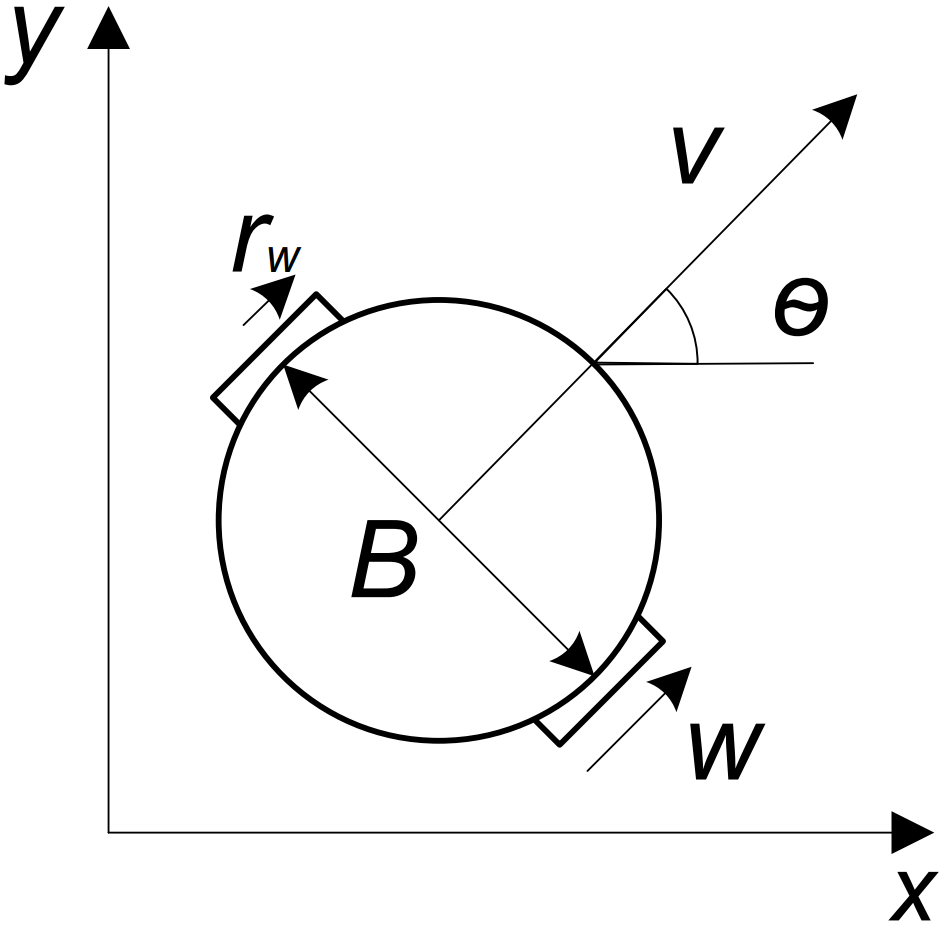
\includegraphics[width=0.27\textwidth]{2_robot}
\begin{center}{\footnotesize Рис. 3: Кинематическая схема мобильного робота}\end{center}
\end{figure}

Метод прост в реализации, так как реализован на языке программирования Python и был протестирован на модели. Результаты моделирования показывают, что метод успешно и эффективно планирует траектории движения группы роботов в неизвестной среде с препятствиями.

Вот некоторые из ключевых особенностей этого метода:
\begin{itemize}
\item \textbf{Децентрализованный} --- это означает, что каждый робот в группе самостоятельно планирует свою собственную траекторию. Это делает метод масштабируемым для больших групп роботов.
\item \textbf{Предотвращение столкновений}: метод использует информацию о расположении препятствий, чтобы избежать столкновений между роботами.
\item \textbf{Безопасность}: метод гарантирует, что роботы не будут подходить слишком близко друг к другу, что может предотвратить столкновения и другие проблемы.
\item \textbf{Эффективность} с точки зрения вычислительных ресурсов.
\end{itemize}

Этот метод потенциально может использоваться в различных областях применения, таких как поисково-спасательные работы, ликвидация последствий стихийных бедствий и мониторинг окружающей среды.

Что касается ограничений этого метода:
\begin{itemize}
\item \textbf{Гарантированно работает только в закрытых помещениях.} В открытой среде роботы могут быть не в состоянии взаимодействовать друг с другом, что может привести к столкновениям.
\item \textbf{Не гарантирует нахождения кратчайшего пути между начальной и конечной точками.} Метод находит путь, который позволяет избежать препятствий и гарантирует, что роботы не подойдут слишком близко друг к другу. Однако этот путь может быть не самым коротким из возможных.
\item\textbf{Не гарантируется, что этот метод будет работать во всех средах.} Этот метод был протестирован в ходе моделирования, но не ясно, насколько хорошо он будет работать в реальных условиях.
\end{itemize}

В целом, метод похож на многообещающий подход для планирования траектории движения группы мобильных роботов в неизвестной среде. Он прост в реализации, эффективен с точки зрения вычислительных ресурсов и при моделировании. Однако имеются некоторые ограничения --- например, гарантированная работа только в закрытых средах. Дальнейшие исследования могли бы быть сосредоточены на устранении этих ограничений.

\pagebreak \header{Траекторное управление мобильным роботом в\\условиях неопределенности \cite{3}}

В статье рассматривается задача управления движением мобильного робота по заданной плавной траектории. Авторы предлагают новый метод расчета минимального расстояния от робота до траектории и робастный регулятор на основе метода последовательного компенсатора. Контроллер обеспечивает ограниченную ошибку ориентации и позиционирования и настраивается в соответствии с конкретными требованиями.

Авторы оценивают контроллер в моделировании и показывают, что он способен успешно отслеживать различные траектории, включая прямые линии, кривые и окружности. Контроллер также может обрабатывать возмущения, такие как изменение скорости робота или наличие препятствий.

\begin{figure}[!h]
\centering
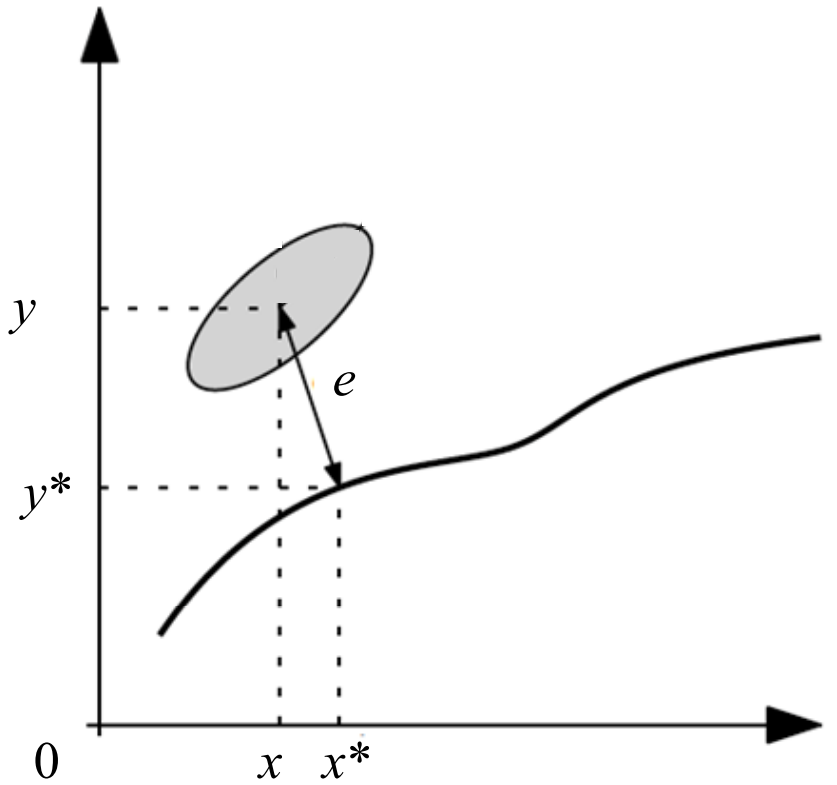
\includegraphics[width=0.27\textwidth]{3_robot}
\begin{center}{\footnotesize Рис. 4: Мобильный робот, движущийся по траектории,\\ представленной гладкой кривой}\end{center}
\end{figure}

Авторы делают вывод, что предлагаемый контроллер является перспективным подходом для управления движением мобильных роботов. Контроллер надежен, прост в реализации и может быть настроен в соответствии с конкретными требованиями.

Ещё несколько выводов, которыми авторы делятся с нами в статье:
\begin{itemize}
\item Использование нелинейного наблюдателя для оценки минимального расстояния от робота до траектории является новым подходом. Наблюдатель способен точно оценить расстояние даже при наличии шума и помех.
\item Контроллер последовательного компенсатора — это простой и эффективный способ управления движением робота. Контроллер способен точно отслеживать траекторию и избегать препятствий.
\item Контроллер оценивался в моделировании, но было бы интересно посмотреть, как он работает в реальных экспериментах.
\end{itemize}

В целом в статье представлен перспективный подход к управлению движением мобильных роботов. Контроллер надежен, прост в реализации и может быть настроен в соответствии с конкретными требованиями.

\pagebreak
\header{Навигация мобильного робота на основе методов\\лазерной дальнометрии \cite{4}}

В статье рассматривается проблема навигации мобильных роботов в динамической недетерминированной среде. Авторы предлагают навигационную систему для мобильного робота-спасателя, предназначенного для поиска пострадавших под завалами разрушенных сооружений. Она основана на лидаре, который позволяет роботу строить карту своего окружения и определять собственное положение. Также учитывается движение динамических препятствий, таких как падающие обломки, чтобы избежать столкновений.

\begin{figure}[!h]
\centering
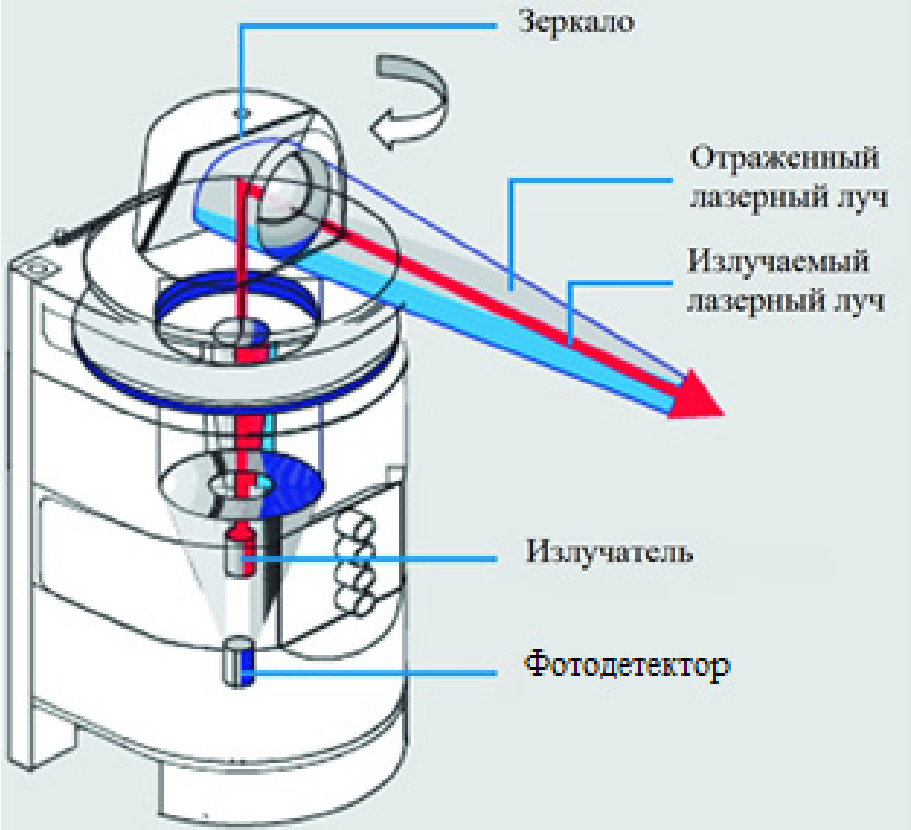
\includegraphics[width=0.4\textwidth]{4_lidar}
\begin{center}{\footnotesize Рис. 5: Типовая конструкция лидара}\end{center}
\end{figure}

Авторы оценили систему в моделировании и показали, что она может успешно перемещаться в различных средах, включая загроможденные комнаты и поля с щебнем. Система также смогла избежать столкновений с динамическими препятствиями.

Исследователи приходят к выводу, что предлагаемая навигационная система является многообещающим подходом для мобильных роботов, работающих в динамических средах. Система надежна и может использоваться в различных приложениях, таких как поисково-спасательные работы, помощь при стихийных бедствиях и производство.

Вот к каким выводам можно прийти, прочитав статью:
\begin{itemize}
\item Использование лидара является многообещающим подходом к навигации мобильных роботов. Лидар может предоставить точную и достоверную информацию об окружающей среде, которая необходима для навигации в динамичных средах.
\item Перспективен и подход авторов к учету движения динамических препятствий. Это сложная проблема, но подход авторов кажется эффективным.
\end{itemize}

В целом, в статье представлен многообещающий подход к навигации мобильных роботов в динамических средах. Система надежна и может использоваться в различных приложениях.

\pagebreak

\header{Силомоментное очувствление электромеханического манипулятора \cite{5}}

Системы измерения силы и момента --- это устройства, которые измеряют силы и моменты, воздействующие промышленным роботом на объекты, с которыми он взаимодействует. Эти системы используются для повышения безопасности и производительности роботов путем обеспечения обратной связи о прилагаемых силах и моментах.

Существует два основных типа систем измерения силы и момента: контактные и бесконтактные. Контактные датчики используют физический контакт с объектом для измерения прилагаемых сил и моментов. Бесконтактные датчики используют такие датчики, как камеры или лазеры, для измерения расстояния и скорости робота и объекта, а затем используют эту информацию для расчета прилагаемых сил и моментов.
Контактные датчики более точны, чем бесконтактные, но они также могут повредить манипулируемый объект. Бесконтактные датчики менее точны, но они безопаснее и могут использоваться для манипулирования деликатными объектами.

Выбор системы измерения силы и момента зависит от области применения. Для применений, где безопасность имеет решающее значение, например, в автомобильной промышленности, часто используются контактные датчики. Для применений, где точность важнее, к примеру, в полупроводниковой промышленности, часто используются бесконтактные датчики.

Системы измерения силы и момента являются важной частью современных промышленных роботов. Они повышают безопасность и производительность роботов, обеспечивая обратную связь о прилагаемых силах и моментах. Эта обратная связь может быть использована для предотвращения столкновений, повреждения объектов и травм операторов.

Преимущества систем измерения силы и момента:
\begin{itemize}
\item \textbf{Повышенная безопасность}: системы измерения силы и момента могут помочь предотвратить столкновения, обеспечивая обратную связь о прилагаемых силах и моментах. Это может помочь защитить операторов и объекты от повреждений.
\item \textbf{Улучшенная производительность}: системы измерения силы и момента могут помочь улучшить производительность роботов, обеспечивая обратную связь о прикладываемых силах и моментах. Это может помочь роботам манипулировать объектами более точно и безопасно.
\item \textbf{Повышенная гибкость}: системы измерения силы и момента могут сделать роботов более гибкими, позволяя им взаимодействовать с более широким спектром объектов.
\end{itemize}

Недостатки систем измерения силы и момента:
\begin{itemize}
\item \textbf{Стоимость}: системы крайне дорогостоящие.
\item \textbf{Сложность}: системы могут быть сложными в установке и обслуживании.
\item \textbf{Точность}: они менее точные, чем датчики других типов, такие как датчики зрения.
\end{itemize}

Системы измерения силы и момента являются важной частью современных промышленных роботов. Они повышают безопасность и производительность роботов, обеспечивая обратную связь о прилагаемых силах и моментах. Эта обратная связь может быть использована для предотвращения столкновений, повреждения объектов и травм операторов.

Однако системы измерения силового момента не лишены своих недостатков. Они могут быть дорогими, сложными и менее точными, чем датчики других типов. Несмотря на эти недостатки, системы измерения силы и момента являются ценным инструментом для повышения безопасности и производительности промышленных роботов.

\pagebreak

\header{Исследование нейронных сетей для обнаружения объектов\\в задаче управления автономным транспортным средством \cite{6}}

Автономная навигация беспилотных транспортных средств — сложная задача, имеющая множество потенциальных применений. Например, автономные транспортные средства можно использовать для доставки посылок, проверки инфраструктуры или даже исследования опасных или удаленных сред. Один из подходов к автономной навигации заключается в использовании обнаружения объектов для определения ориентиров в окружающей среде. Эту задачу можно выполнить при помощи различных методов, включая глубокое обучение. В этой статье авторы исследуют использование системы обнаружения объектов YOLO v2 для автономной навигации.

YOLO v2 — это система глубокого обучения, которая может обнаруживать объекты на изображениях с высокой скоростью. Она может обнаруживать объекты за один проход по изображению, это делает ее хорошо подходящей для приложений реального времени, таких как автономная навигация.

В этой статье авторы обучили систему YOLO v2 обнаруживать ориентиры в наборе данных изображений, сделанных с транспортного средства. Система способна обнаруживать ориентиры с высокой точностью даже в сложных условиях, таких как плохое освещение и затенение. Затем они использовали систему YOLO v2 для управления транспортным средством в смоделированной среде. Транспортное средство может передвигаться автономно, объезжая препятствия и благополучно добираясь до места назначения.

Результаты этой статьи демонстрируют, что YOLO v2 является многообещающим подходом к автономной навигации. Система способна обнаруживать ориентиры с высокой точностью даже в сложных условиях. Это делает ее хорошо подходящей для реальных приложений, таких как доставка посылок или проверка инфраструктуры.

\begin{table}[h!]
\centering
\begin{tabular}{|m{3cm}||m{1.8cm}|m{2cm}|m{2.9cm}|m{1.9cm}|} 
\hline
\begin{center}Сеть\end{center} & MobileNet & Tiny YOLO\newline (с нуля) & Tiny YOLO\newline (предобученная) & Full YOLO \\ 
\hline
\hline
Размер входа & 1024$\times$768 & 960$\times$544 & 102$\times$768 & 1024$\times$768 \\ 
\hline
Качество (mAP) на первом наборе & 0.4765 & 0.5294 & 0.4126 & 0.5566 \\ 
\hline
Качество (mAP) на втором наборе & 0.4936 & 0.4246 & 0.5576 & 0.7053 \\ 
\hline
\end{tabular}
\begin{center}{\footnotesize Табл. 1: Результаты тестирования архитектур нейронных сетей}\end{center}
\end{table}

В статье авторы представили метод автономной навигации беспилотных транспортных средств с использованием YOLO v2. При помощи этого метода в будущем планируется решить задачи по улучшению обнаружения объектов, планированию траектории и контролю. Мы считаем, что, решая эти задачи, можно разработать полностью автономное транспортное средство, способное безопасно передвигаться в самых разных условиях.

\header{Заключение}

В заключении следует сказать, что изучение и развитие приведенных тем имеют немаловажное значение для развития робототехнических систем управления. Полученные результаты и методы могут быть применены в различных областях, таких как производство, автономная навигация, медицина и другие. Дальнейшие исследования в этих областях могут привести к новым достижениям и применению роботов в ещё более широком спектре задач.

\printbibliography[title={\centering Список литературы}]

\end{document}